\documentclass[12pt]{article}
\usepackage[utf8]{inputenc}
\usepackage[spanish,es-lcroman, es-tabla]{babel}
\usepackage[autostyle,spanish=mexican]{csquotes}
\usepackage{amsmath}
\usepackage{amssymb}
\usepackage{nccmath}
\numberwithin{equation}{section}
\usepackage{amsthm}
\usepackage{graphicx}
\usepackage{epstopdf}
\DeclareGraphicsExtensions{.pdf,.png,.jpg,.eps}
\usepackage{color}
\usepackage{float}
\usepackage{multicol}
\usepackage{enumerate}
\usepackage[shortlabels]{enumitem}
\usepackage{anyfontsize}
\usepackage{anysize}
\usepackage{array}
\usepackage{multirow}
\usepackage{enumitem}
\usepackage{cancel}
\usepackage{tikz}
\usepackage{circuitikz}
\usepackage{tikz-3dplot}
\usetikzlibrary{babel}
\usetikzlibrary{shapes}
\usepackage{bm}
\usepackage{mathtools}
\usepackage{esvect}
\usepackage{hyperref}
\usepackage{relsize}
\usepackage{siunitx}
\usepackage{physics}
%\usepackage{biblatex}
\usepackage{standalone}
\usepackage{mathrsfs}
\usepackage{bigints}
\usepackage{bookmark}
\spanishdecimal{.}

\setlist[enumerate]{itemsep=0mm}

\renewcommand{\baselinestretch}{1.5}

\let\oldbibliography\thebibliography

\renewcommand{\thebibliography}[1]{\oldbibliography{#1}

\setlength{\itemsep}{0pt}}
%\marginsize{1.5cm}{1.5cm}{2cm}{2cm}


\newtheorem{defi}{{\it Definición}}[section]
\newtheorem{teo}{{\it Teorema}}[section]
\newtheorem{ejemplo}{{\it Ejemplo}}[section]
\newtheorem{propiedad}{{\it Propiedad}}[section]
\newtheorem{lema}{{\it Lema}}[section]

\usepackage{mathrsfs}
%\usepackage{enumerate}
%\author{M. en C. Gustavo Contreras Mayén. \texttt{curso.fisica.comp@gmail.com}}
\title{Funciones ortogonales \\ {\large Tema 3 - Matemáticas Avanzadas de la Física}}
\date{ }
\begin{document}
%\renewcommand\theenumii{\arabic{theenumii.enumii}}
\renewcommand\labelenumii{\theenumi.{\arabic{enumii}}}
\maketitle
\fontsize{14}{14}\selectfont
\section{Ecuaciones diferenciales auto-adjuntas.}
Ya hemos abordado y manejado ecuaciones diferenciales de segundo orden, cuya forma general en términos de un operador lineal diferencial de segundo orden ($\mathscr{L}$) es
\begin{equation}
\mathscr{L} u(x) = \left( p_{0}(x) \dfrac{d^{2}}{d x^{2}} + p_{1}(x) \dfrac{d}{dx} + p_{2}(x) \right)  u(x)
\label{eq:ecuacion_1}
\end{equation}
Donde reconocemos que $P(x) = p_{1}(x)/p_{0}(x)$ y $Q(x)= p_{2}(x)/p_{0}(x)$.
\\
Revisaremos la ecuación diferencial en algún intervalo cerraro $[a,b]$ y que las funciones $p_{0}$, $p_{1}$, y $p_{2}$ son funciones reales de $x$ dentro de una región de interés $a \leq x \leq b$, las primeras $2-i$-derivadas de $p_{i}(x)$ son continuas. Además, $p_{0}$ no se anula en $a<x<b$. Los ceros de $p_{0}$ son puntos singulares, podemos elegir el intervalo $[a,b]$ de tal manera que no hayan puntos singulares al interior del intervalo, sucede a menudo que puedan existir puntos singulares en las fronteras.
\\
Se define el operador adjunto $\overline{\mathscr{L}}$ como
\begin{eqnarray}
\begin{aligned}
\overline{\mathscr{L}} u &= \dfrac{d^{2}}{d x^{2}}[ p_{0} u] - \dfrac{d}{dx} [p_{1} u] + p_{2} u \\
&= p_{0}\dfrac{d^{2} u}{d x^{2}} + (2 p'_{0} - p_{1}) \dfrac{du}{dx} + (p''_{0} - p'_{1} + p_{2}) u
\label{eq:ecuacion_2}
\end{aligned}
\end{eqnarray}
Comparando las ecuaciones (\ref{eq:ecuacion_1}) y (\ref{eq:ecuacion_2}), la condición necesaria y suficiente para que $\mathscr{L} = \overline{\mathscr{L}}$ es que
\begin{equation}
p'_{0}(x) = \dfrac{d p_{0}(x)}{dx} = p_{1}(x) \label{eq:ecuacion_3}
\end{equation}
Cuando la condición se satisface
\begin{equation}
\overline{\mathscr{L}} u = \mathscr{L} = \dfrac{d}{dx} \left[ p(x) \dfrac{d u(x)}{dx} \right] + q(x) u(x)
\label{eq:ecuacion_4}
\end{equation}
y se dice que el operador $\mathscr{L}$ es un \emph{auto-adjunto}. Cuando tenemos el caso del autoadjunto, $p_{0}(x)$ queda reemplazado por $p(x)$ y a la vez, $p_{2}(x)$ se reemplaza por $q(x)$, ya no hay necesidad de usar los subíndices.
\\
De lo que hemos revisado en el curso, la ecuación de Legendre y la ecuación del oscilador lineal, son autoadjuntas, mientras que las ecuaciones de Laguerre y Hermite, no lo son. De manera general, de la teoría de las ecuaciones diferenciales autoadjuntas de segundo orden, podemos transformar siempre, un operador no auto-adjunto a una forma auto-adjunta.
\\
Sea la ecuación (\ref{eq:ecuacion_1}) tal que $p'_{0}\neq p_{1}$, si multiplicamos $\mathscr{L}$ por
\[ \dfrac{1}{p_{0} (x)} \exp \left[ \int^{x} \dfrac{p_{1}(t)}{p_{0}(t)} dt \right] \]
se obtiene
\begin{equation}
\begin{split}
\dfrac{1}{p_{0} (x)} \exp \left[ \int^{x} \dfrac{p_{1}(t)}{p_{0}(t)} dt \right] \mathscr{L} u (x) &= \dfrac{d}{dx} \left\lbrace \exp \left[ \int^{2} \dfrac{p_{1}(t)}{p_{0}(t)} dt \right] \dfrac{du(x)}{dx} \right\rbrace \\
&+ \dfrac{p_{2}(x)}{p_{0}(x)} \cdot \exp \left[ \dfrac{p_{1}(t)}{p_{0}(t)} \right] u
\end{split}
\end{equation}
que como se nota, no es autoadjunta. Veamos que aparece $p_{0}(x)$ en el denominador, por lo que se requiere que $p_{0}(x) \neq 0, a < x < b$. Supondremos en adelante que $\mathscr{L}$ se muestra como auto-adjunto.
\section{Funciones propias, valores propios.}
Del tema de separación de variables (o del problema físico), podemos expresar una ecuación diferencial de segundo orden de la forma
\begin{equation}
\mathscr{L} u(x) =  \lambda w(x) u(x) = 0
\label{eq:ecuacion_6}
\end{equation}
donde
\begin{enumerate}
\item $\lambda$ es una constante.
\item $w(x)$ es una función conocida de $x$, llamada función de peso o de densidad.
\item Se necesita que $w(x)>0$, excepto en puntos aislados en los cuales $w(x)=0$.
\end{enumerate}
Para un valor dado de $\lambda$, una función $u_{\lambda}(x)$ que satisface la ecuación (\ref{eq:ecuacion_6}) y las condiciones de frontera definidas, ya le habíamos dado el nombre de \emph{función propia} que corresponde a $\lambda$. La constante $\lambda$, es el \emph{valor propio}.
\\
Como tal, no hay garantía de que una función propia $u_{\lambda}(x)$ exista para un determinado $\lambda$, por tanto, para que exista una función propia, debe de cumplir la restricción de ciertos valores de $\lambda$ en un conjunto discreto. Lo que sería un versión matemática de la cuantización en física:
\[ H \psi (x) =  E \psi (x) \]
donde el operador diferencial $\mathscr{L}$ es el Hamiltoniano $H$ y el valor propio $(-\lambda)$ es la energía total $E$ del sistema. La función $\psi (x)$ es la función de onda.
\\
\textbf{Ejemplo:} Ecuación de Legendre.
\begin{equation}
(1-x^{2}) y'' - 2xy' + n(n+1) y = 0 \label{eq:ecuacion_7}
\end{equation}
De las ecuaciones (\ref{eq:ecuacion_1}) y (\ref{eq:ecuacion_6}), tenemos que
\begin{eqnarray}
\begin{aligned}
p_{0}(x) &= 1 - x^{2} = p \hspace{2cm} w(x) =  1 \\
p_{1}(x) &= -2x = p' \hspace{2cm} \lambda = n(n+1) \\
p_{2}(x) &= 0 = q
\end{aligned}
\end{eqnarray}
La solución diverge a menos que $n$ esté restringida a un valor entero, por lo que podemos decir que hay una cuantización de los valores de $\lambda$.
\\
\textbf{Ejemplo: Deuterón.}
Para profundizar un poco más en los conceptos de funciones propias y valores propios, consideremos un modelo simple del deuterón. La interacción nuclear neutrón-protón la podemos representar por un pozo cuadrado de potencial:
\begin{equation*}
V = \begin{cases}
V_{0} < 0 \hspace{0.5cm} \text{para } 0 \leq r < a \\
V = 0 \hspace{0.5cm} \text{para } r > a
\end{cases}
\end{equation*}
la ecuación de Schröndinger es
\begin{equation}
- \dfrac{\hbar^{2}}{2M} \nabla^{2} \psi + V \psi =  E \psi
\label{eq:ecuacion_9}
\end{equation}
con $\psi =  \psi(r)$, podemos escribir $u(r) = r \psi (r)$
podemos representar la ecuación como
\begin{equation}
\dfrac{d^{2} u}{d r^{2}} + k_{1}^{2} u = 0
\label{eq:ecuacion_10}
\end{equation}
donde
\begin{equation}
k_{1}^{2} =  \dfrac{2M}{\hbar} (E - V_{0}) > 0
\label{eq:ecuacion_11}
\end{equation}
para el interior de la región $0 \leq r < a$. En la ecuación, $M$ es la masa reducida del sistema protón-neutrón. Para $a < r < \infty$, tenemos
\begin{equation}
\dfrac{d^{2} u}{d r^{2}} - k_{2}^{2} u = 0
\label{eq:ecuacion_12}
\end{equation}
con
\begin{equation}
k_{2}^{2} = - \dfrac{2ME}{\hbar^{2}} > 0
\label{eq:ecuacion_13}
\end{equation}
De la condición de frontera que permite $\psi$ sea finito, $u(0)=0$ y
\begin{equation}
u_{1}(r) =  \sin k_{1} r, \hspace{1.5cm} 0 \leq r < a
\label{eq:ecuacion_14}
\end{equation}
Fuera del pozo de potencial, tenemos una combinación lineal de dos exponenciales
\begin{equation}
u_{2}(r) = A \exp k_{2} r + B \exp(-k_{2} r) \hspace{1.5cm} a < r < \infty
\label{eq:ecuacion_15}
\end{equation}
Hay dos condiciones que hacen que $u_{1}(a) = u_{2}(a)$ y $u'_{1}(a) = u'_{2}(a)$, éstas condiciones nos dan
\begin{eqnarray}
\begin{aligned}
\sin k_{1} a &= A \exp	k_{2} a + B \exp(-k_{2}a) \\
k_{1} \cos k_{1} a &= k_{2} A \exp k_{2} a - k_{2} B \exp(-k_{2}a)
\label{eq:ecuacion_16}
\end{aligned}
\end{eqnarray}
La condición de que nos permite tener una combinación protón-neutrón es tal que $\int \psi* \psi d \tau = 1$. Esta condición resulta de la imposición en la condición de frontera, la que hace que $\psi(r)$ sea finita mientras $r \to \infty$. Así pues, significa que $A=0$, al dividir las dos ecuaciones (para cancelar $B$), se obtiene
\begin{equation}
\tan k_{1} a = - \dfrac{k_{1}}{k_{2}} = - \sqrt{\dfrac{E - V_{0}}{-E}} 
\label{eq:ecuacion_17}
\end{equation}
que es una ecuación relevante de la energía $E$ que tiene un conjunto \emph{discreto} de soluciones:
\begin{enumerate}
\item Si $E$ es tal que satisface la ecuación (\ref{eq:ecuacion_17}), las soluciones $u_{1}(r)$ y $u_{2}(r)$ satisfacen las condiciones de frontera.
\item Si la ecuación (\ref{eq:ecuacion_17}) no se satisface, no existe una solución aceptable.
\end{enumerate}
Los valores de $E$ para los cuales la ecuación (\ref{eq:ecuacion_17}) se satisface, corresponde a los valores propios, las funciones $u_{1}$ y $u_{2}$ (o $\psi$) son las funciones propias. En este ejercicio del deuterón, hay un (y sólo un) valor negativo de $E$ que satisface la ecuación (\ref{eq:ecuacion_17}), es decir, sólo tiene un estado base.
\\
Pero qué ocurre si $E$ no satisface la ecuación (\ref{eq:ecuacion_17})? si $E$ no tiene un valor propio?
\\
Gráficamente podemos imaginarnos $E$ y por tanto $k_{1}$ varían suavemente.
\begin{figure}[!h]
\centering
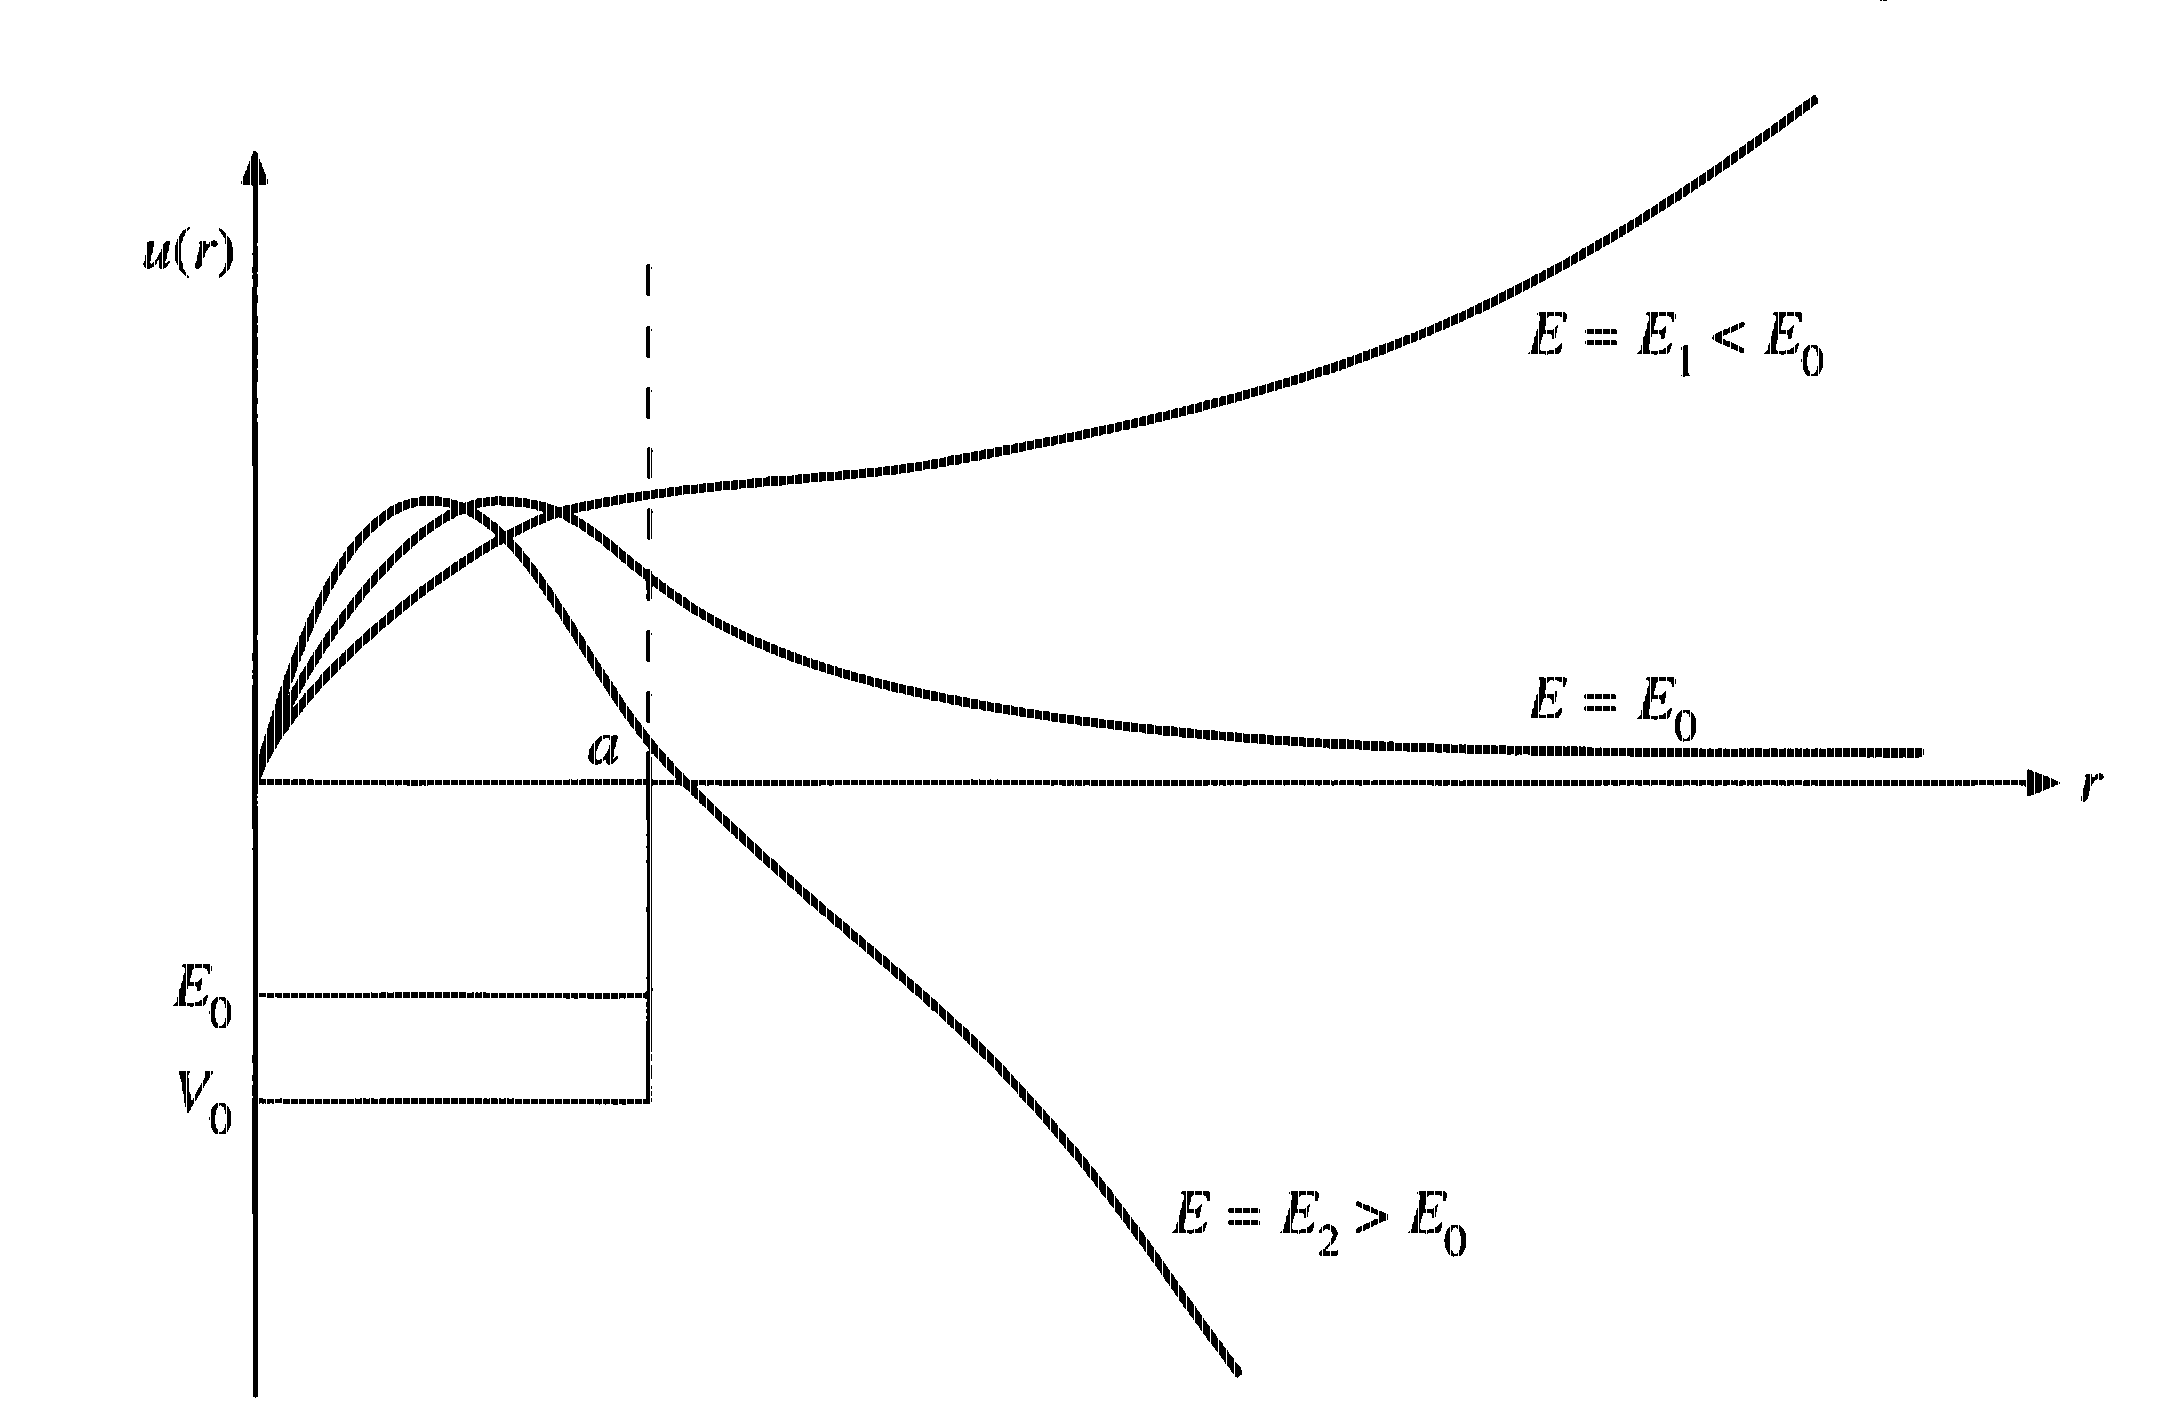
\includegraphics[scale=1]{Tema3_01.eps} 
\end{figure}
\begin{itemize}
\item Para $E= E_{1} < E_{0}$, $k_{1}$ se reduce y $\sin k_{1}a$ no se modifica mucho. Pero las condiciones de unión (ecuación \ref{eq:ecuacion_16}), pide que $A>0$, por lo que la función de onda tiene a $+\infty$ de manera exponencial.
\item Para $E=E_{2} > E_{0}$, $k_{1}$ es grande,  y $\sin k_{1}a$ tiene rápidamente un pico y luego decae más rápido que $r=a$. Las condiciones de unión, piden que $A<0$, por lo que la función de onda tiene a $-\infty$ exponencialmente.
\item Para $E=E_{0}$ un valor propio permite que la función de onda tenga un comportamiento exponencial negativo asintótico.
\end{itemize}
\section{Condiciones de frontera.}
En la definición de función propia, hemos ocmentado que $u_{\lambda} (x)$ requiere satisfacer ciertas condiciones de frontera. Tales condiciones de frontera, pueden presentarse en tres modos:
\begin{enumerate}
\item \textbf{Condiciones de Cauchy. } El valor de una función y su derivada, se especifican en la frontera. 
\item \textbf{Condiciones de Dirichlet. }El valor de una función se especifica en la frontera.
\item \textbf{Condiciones de Neumann. } La derivada normal (gradiente) de una función se especifica en la frontera.
\end{enumerate}
El término condiciones de frontera considera el caso especial del concepto de condiciones inciales, por ejemplo, determinamos la posición inicial $x_{0}$ y la velocidad inicial $v_{0}$ para algún problema con condiciones de Cauchy de frontera. La única diferencia en el uso de las condiciones de frontera en los casos unidimensionales, es que debemos aplicar las condiciones en ambos extremos del intervalo.
\\
Normalmente la manera en que la ecuación diferencial o las condiciones de frontera en las soluciones se garantizan que e los extremos de nuestro intervalo (es decir, la frontera), los siguientes productos se anulen
\begin{eqnarray}
\begin{aligned}
p(x) v*(x) \dfrac{d u(x)}{dx} \vert_{x=a} = 0 \\
p(x) v*(x) \dfrac{d u(x)}{dx} \vert_{x=b} = 0
\label{eq:ecuacion_18}
\end{aligned}
\end{eqnarray}
Donde $u(x)$ y $v(x)$ son soluciones de la ecuación diferencial (\ref{eq:ecuacion_6}). Podemos de cualquier forma, trabajar con un conjunto de condiciones de frontera menos restrictivas:
\begin{equation}
v* p u' \vert_{x=a} =  v* p u' \vert_{x=b} \label{eq:ecuacion_19}
\end{equation}
donde $u(x)$ y $v(x)$ son soluciones de la ecuación diferencial correspondiente al mismo valor propio o a uno diferente. 
\\
Las ecuaciones (\ref{eq:ecuacion_18}) y (\ref{eq:ecuacion_19}) se escriben en términos de $v*$ como conjugado complejo. Cuando las soluciones son reales $v=v*$, podemos omitir el asterisco. En las expansiones exponenciales de Fourier y en ejercicios de mecánica cuántica, las funciones serán complejas y se requiere el conjugado complejo.
\\
Esas propiedades (ecuaciones \ref{eq:ecuacion_18} y \ref{eq:ecuacion_19}) son importantes para definir el concepto de operador Hermitianoy la consecuencia de que podemos elegir el intervalo $(a,b)$, que nos asegure que la ecuación (\ref{eq:ecuacion_18}) o (\ref{eq:ecuacion_19}) se satisfacen.
\\
\textbf{Ejemplo: Elección del intervalo de integración.}
\\
Para $\mathscr{L} = d^{2}/dx^{2}$ una posible ecuación de valores propios es
\begin{equation}
\dfrac{d^{2}}{d x^{2}} y(x) + n^{2} y(x) = 0 \label{eq:ecuacion_20}
\end{equation}
con funciones propias
\[ \begin{split}
u_{n} &= \cos nx \\
v_{m} &= \sin mx
\end{split} \]
La ecuación (\ref{eq:ecuacion_19}) es
\begin{eqnarray*}
- n \sin mx \sin nx \vert^{b}_{a} &= 0 \nonumber \\
\text{intercambiando $u_{n}$ y $v_{m}$} \nonumber \\
m \cos mx \cos nx \vert^{b}_{a} &= 0 
\end{eqnarray*}
Ya que $\sin mx$ y $\cos nx$ son periódicos, con período $2 \pi$ (con $n$ y $m$ enteros), la ecuación (\ref{eq:ecuacion_19}) se satisface si $a=x_{0}$ y $b= x_{0} + 2 \pi$. El intervalo se elige tal que las condiciones de frontera se satisfacen.
\\
Para el ejemplo (series de Fourier), los valores comunes son $x_{0}=0$ que conducen a $(0, 2 \pi)$ y $x_{0} = - \pi$, que conducen a $(-\pi, \pi)$
\begin{center}
\begin{tabular}{l c c c}
\hline \\
Ecuación & $a$ & $b$ & $w(x)$ \\ \hline
Legendre & $-1$ & $1$ & $1$ \\ \hline
Modificados Legendre & $0$ & $1$ & $1$ \\ \hline
Asociados Legendre & $-1$ & $1$ & $1$ \\ \hline
Chebychev I & $-1$ & $1$ & $(1-x^{2})^{-1/2}$ \\ \hline
Modificados Chebychev & $0$ & $1$ & $[x(1-x)]^{-1/2}$ \\ \hline
Chebychev II & $-1$ & $1$ & $(1-x^{2})^{1/2}$ \\ \hline
Laguerre & $0$ & $\infty$ & $e^{-x}$ \\ \hline
Asociados Laguerre & $0$ & $\infty$ & $x^{k} e^{-x}$ \\ \hline
Hermite & $-\infty$ & $\infty$ & $e^{-x^{2}}$ \\ \hline
Oscilados armónico & $0$ & $2 \pi$ & $1$ \\ \hline
\end{tabular}
\end{center}
\section{Operadores hermitianos.}
Veamos una propiedad importante que se obtiene al combinar un operador diferencial de segundo orden auto-adjunto (ecuación \ref{eq:ecuacion_6}) más soluciones $u(x)$ y $v(x)$, que satisfacen las condiciones de frontera dadas por la ecuación (\ref{eq:ecuacion_19}).
\\
Integramos el producto de $v*$ (conjugado complejo) con el operador diferencial auto-adjunto de segundo order $\mathscr{L}$ (operando sobre $u$) en el intervalo $a \leq x \leq b$, usando la ecuación (\ref{eq:ecuacion_4}):
\begin{equation}
\int_{a}^{b} v* \mathscr{L} u dx = \int_{a}^{b} v* (pu')' dx + \int_{a}^{b} v* qu dx
\label{eq:ecuacion_21}
\end{equation}
Integrando por partes, obtenemos
\begin{equation}
\int_{a}^{b} v*(pu')' dx = v* pu' \bigg\vert_{a}^{b} - \int_{a}^{b} v*' pu' dx
\label{eq:ecuacion_22}
\end{equation}
con las condiciones de frontera, el término integrado se anula (ecuación \ref{eq:ecuacion_19}), al integrar el término que queda, ahora por partes nuevamente, tenemos que
\begin{equation}
- \int_{a}^{b} v*' pu' dx = - v*' pu \bigg\vert_{a}^{b} + \int_{a}^{b} u(pv*')' dx
\label{eq:ecuacion_23}
\end{equation}
El término integrado, se anula nuevamente al considerar la ecuación (\ref{eq:ecuacion_19}). Una combinación de las ecuaciones (\ref{eq:ecuacion_21}) a la (\ref{eq:ecuacion_23}), nos resulta
\begin{equation}
\int_{a}^{b} v* \mathscr{L} u dx = \int_{a}^{b} u \mathscr{L} v* dx
\label{eq:ecuacion_24}
\end{equation}
Esta propiedad nos dice que el operador $\mathscr{L}$ es Hermitiano respecto a las funciones $u(x)$ y $v(x)$ con la que satisface las condiciones de frontera, que se especifican por la ecuación (\ref{eq:ecuacion_19}). Hay que tomar en cuenta que ésta propiedad hermitiana, es consecuencia de ser auto-adjunto más las condiciones de frontera.
\section{Operadores hermitianos en mecánica cuántica.}
Generalizando la teoría de operadores hermitianos en mecánica cuántica, podemos agregar que: los operadores no pueden ser operadores de segundo orden y tampoco pueden ser reales. $p_{x} = - i \hbar(\partial / \partial x)$ sería un operador Hermitiano.
\\
Podemos suponer (como en realidad se acostumbra en mecánica cuántica) que las funciones de onda satisfacen las condiciones de frontera: se anulan cuando tienden a infinito o tienen un comportamiento periódico.
\\
El operador $\mathscr{L}$ se denomina \emph{Hermitiano}, si
\begin{equation}
\int \psi_{1}* \mathscr{L} \psi_{2} d \tau =  \int (\mathscr{L} \psi_{1})* \psi_{2} d \tau
\label{eq:ecuacion_25}
\end{equation}
El adjunto $A^{\dagger}$ de un operador $A$ se define como 
\begin{equation}
\int \psi_{1}* A^{\dagger} \psi_{2} d \tau = \int (A \psi_{1})* \psi_{2} d \tau
\label{eq:ecuacion_26}
\end{equation}
Aquí hay una pequeña diferencia de la definición clásica del operador de segundo orden (ecuación \ref{eq:ecuacion_2}), el ajunto está definido en términos de la integral, con $A^{\dagger}$ como parte del integrando. Si $A=A^{\dagger}$ (auto-adjunto), entonces $A$ es Hermitiana. Al revés no es tan sencillo (y no siempre cierto), pero en mecánica cuántica los términos \emph{auto-adjunto} y \emph{Hermitiano}, se usan como sinónimos.
\\
El valor esperado de un operador $\mathscr{L}$ se define como
\begin{equation}
< \mathscr{L} > = \int	\psi* \mathscr{L} \psi d \tau
\label{eq:ecuacion_27a}
\end{equation}
En el ámbito de mecánica cuántica $< \mathscr{L} >$ corresponde al resultado de una medición de una cantidad física representada por $\mathscr{L}$ donde el sistema físico es un estado descrito por la función de onda $\psi$. Si queremos que $\mathscr{L}$ sea Hermitiano, debemos de mostrar que $<\mathscr{L}>$ es real (en correspondencia de una medición en física). Tomando el conjugado complejo de la ecuación (\ref{eq:ecuacion_27a}), tenemos
\[ \begin{split}
< \mathscr{L} >* &= \left[ \int \psi* \mathscr{L} \psi d \tau \right] \\
&= \int \psi \mathscr{L}* \psi * d \tau
\end{split} \]
Ordenando los factores en el integrando, resulta
\[ < \mathscr{L} >* = \int (\mathscr{L} \psi )* \psi d \tau \]
De la definición de operador Hermitiano (ecuación \ref{eq:ecuacion_25})
\begin{equation}
< \mathscr{L} >* = \int \psi* \mathscr{L} \psi d \tau = < \mathscr{L} > 
\label{eq:ecuacion_27b}
\end{equation}
o $< \mathscr{L} >$ es real.
\section{Operadores Hermitianos (auto-adjuntos).}
Los operadores hermitianos o auto-adjuntos tienen tres propiedades de gran importancia en la física tanto clásica como cuántica.
\begin{enumerate}
\item Los valores propios de un operador hermitiano son reales.
\item Las funciones propias de un operador hermitiano son ortogonales.
\item Las funciones propias de un operador hermitiano forman un conjunto completo.
\end{enumerate}
\subsection{Valores propios reales.}
Sea
\begin{equation}
\mathscr{L} u_{i} + \lambda_{i} w u_{i} = 0
\label{eq:ecuacion_28}
\end{equation}
Suponemos la existencia de un segundo valor propio y función propia
\begin{equation}
\mathscr{L} u_{j} + \lambda_{j} w u_{j} = 0
\label{eq:ecuacion_29}
\end{equation}
Entonces, al tomar el conjugado completo, resulta
\begin{equation}
\mathscr{L} u_{j}* + \lambda_{j}* w u_{j}* = 0
\label{eq:ecuacion_30}
\end{equation}
donde $\mathscr{L}$ es un operador real ($p$ y $q$ son funciones reales de $x$) y $w(x)$ es una función real. Permitimos que tanto $\lambda_{k}$ como $u_{k}$ sean complejos. Multiplicando la ecuación (\ref{eq:ecuacion_28}) y (\ref{eq:ecuacion_30}) por $u_{i}$, y luego se restan, para obtener
\begin{equation}
u*_{j} \mathscr{L} u_{i} - u_{i} \mathscr{L} u*_{j} =  (\lambda*_{j} - \lambda_{i}) w u_{i} u_{j}*
\label{eq:ecuacion_31}
\end{equation}
integramos en el intervalo $a \leq x \leq b$,
\begin{equation}
\int_{a}^{b} u*_{j} \mathscr{L} u_{i} dx - \int_{a}^{b} u_{i} \mathscr{L} u*_{j} dx = (\lambda*_{j} - \lambda_{i}) \int_{a}^{b}  u_{i} u_{j}* w dx
\label{eq:ecuacion_32}
\end{equation}
Como $\mathscr{L}$ es Hermitiano, el lado izquierdo de la igualdad se anula considerando la ecuación (\ref{eq:ecuacion_26}) y tenemos
\begin{equation}
(\lambda*_{j} - \lambda_{i}) \int_{a}^{b}  u_{i} u_{j}* w dx = 0
\label{eq:ecuacion_33}
\end{equation}
Si $i=j$ la integran no se anula ( $w(x) > 0$ para puntos aislados), a menos que tengamos el caso trivial $u_{i}=0$. Por tanto el coeficiente $(\lambda*_{i} - \lambda_{j})$ debe de ser cero
\begin{equation}
\lambda*_{i} = \lambda_{j})
\label{eq:ecuacion_34}
\end{equation}
Lo que es una prueba matemática de que el valor propio es real, ya que $\lambda_{i}$ representa a cualquiera de los valores propios, se cumple esta propiedad.
\\
En mecánica cuántica los valores propios corresponden a cantidades medibles, tales como la energía o el momento angular. Con la teoría revisada en términos de operadores hermitianos, esta prueba de que los valores propios nos garantiza que la teoría predice valores reales para esas cantidades físicas medibles.
\subsection{Funciones propias ortogonales.}
Si tomamos $i \neq	j$ y si $\lambda_{i} \neq \lambda_{j}$ la integral del producto de dos funciones propias diferentes debe de anularse:
\begin{equation}
\int_{a}^{b} u_{i}u*_{j} w dx = 0
\label{eq:ecuacion_35}
\end{equation}
Esta condición es llamada \emph{ortogonalidad}. Se dice que las funciones propias $u_{i}(x)$ y $u_{j}(x)$ son ortogonales con respecto a una función de peso $w(x)$ en el intervalo $[a,b]$.
\\
Si tenemos el caso $i \neq j$ pero se mantiene que $\lambda_{i} = \lambda_{j}$, se tiene el llamado caso \emph{degenerado}. Esto significa que la independencia linea de las funciones propias que corresponden al mismo valor propio, no son automáticamente ortogonales, por lo que deberíamos usar un método que nos permita recuperar el conjunto ortogonal.  Aunque tengamos funciones propias en el caso degenerado y sean no ortogonales, siempre se pueden ortogonalizar.
\\
\textbf{Ejemplo: Series de Fourier.}
\\
Consideremos la ecuación 
\[ \dfrac{d^{2}}{d x^{2}} y(x) + n^{2} y(x) = 0 \]
Que en mecánica cuántica puede describir una partícula en una caja, o puede representar la cuerda de un violín con funciones propias (degeneradas) $\cos nx, \sin nx$.
\\
Con $n$ real, las integrales ortogonales son
\begin{enumerate}[label=\alph*)]
\item $\begin{aligned}[t] \int_{x_{0}}^{x_{0} +  2 \pi} \sin mx \sin nx dx = C_{n} \delta_{nm} \end{aligned} $ 
\item $\begin{aligned}[t] \int_{x_{0}}^{x_{0} +  2 \pi} \cos mx \cos nx dx = D_{n} \delta_{nm} \end{aligned} $ 
\item $\begin{aligned}[t] \int_{x_{0}}^{x_{0} +  2 \pi} \sin mx \cos nx dx = 0 \end{aligned} $
\end{enumerate}
Para un intervalo de $2 \pi$ el análisis previo, garantiza la delta de Kronecker en los incisos a) y b), pero no para el iniciso c), ya que c) involucra funciones propias degeneradas. Pero vemos que en c) siempre se anula para todas las integrales $m$ y $n$.
\\
De la teoría de Sturm-Liouville no nos dice nada sobre los valores de $C_{n}$ y $D_{n}$. Al calcularlos:
\begin{eqnarray*}
C_{n} &= \begin{cases}
\pi  & n \neq 0 \\
0  & n = 0 \end{cases}  \nonumber \\
D_{n} &= \begin{cases}
\pi & n \neq 0 \\
2 \pi & n = 0 \end{cases}
\end{eqnarray*}
La ortogonalidad de los integrandos forma la base para las series de Fourier.
\\
\textbf{Ejemplo: Expansión de funciones propias ortogonales: una onda cuadrada.}
\\
La propiedad de \emph{completez} significa que cierta clase de funciones (funciones continuas por secciones o pedazos), puede representarse por una serie de funciones propias ortogonales, con cualquier grado de precisión. Consideremos la onda cuadrada:
\begin{equation}
f(x) = \begin{cases}
\dfrac{h}{2} & 0 < x < \pi \\
- \dfrac{h}{2} & -\pi < x < o
\end{cases}
\label{eq_ecuacion_36}
\end{equation}
Esta función puede desarrollarse en funciones propias de varios tipos: Legendre, Hermite, Chebyshev, etc. La elección de la función propia se hace en base a la conveniencia del problema. Si elegimos para el desarrollo de la solución, las funciones propias $\cos nx$ y $\sin nx$.
\\
La serie de funciones propias se escribe conveniente (y convencionalmente) como
\[ f(x) = \dfrac{a_{0}}{2} + \sigma_{n=1}^{\infty} (a_{n} \cos nx +  b_{n} \sin nx) \]
De la ortogonalidad de los integrados, los coeficientes están dados por
\begin{eqnarray*}
a_{n} = \dfrac{1}{\pi} \int_{-\pi}^{\pi} f(t) \cos nt dt \\
b_{n} = \dfrac{1}{\pi} \int_{-\pi}^{\pi} f(t) \sin nt dt, \hspace{1cm} n = 0,1,2,\ldots
\end{eqnarray*}
La sustitición directa de $\pm h/2$ para $f(t)$, devuelve que
\[ a_{n} = 0 \]
lo que ya se esperaba dada la antisimetría y además
\[ b_{n} = \dfrac{h}{n \pi} (1 - \cos n \pi) = \begin{cases}
0 & n \text{ par} \\
\dfrac{2h}{n \pi} & n \text{ impar} \end{cases} \]
Por lo que la expansión de las funciones propias (de Fourier) de una onda cuadrada es
\begin{equation}
f(x) = \dfrac{2h}{\pi} \sum_{n=0}^{\infty} \dfrac{\sin(2n+1)x}{(2n+1)}
\end{equation}
\subsection{Degeneración.}
Si $N$ funciones propias linealmente independientes corresponden al mismo valor propio, se dice que el valor propio es $N$-veces degenerado.
\\
Un ejemplo directo lo tomamos de las funciones propias y valores propios en la ecuación del oscilador lineal: para cada valor propio $n$, hay dos posibles soluciones: $\sin x$ y $\cos x$ (y cualquier posibles combinación lineal). En este caso, las funciones son degeneradas o el valor propio es degenerado.
\\
Otro ejemplo es el sistema electrón en un átomo (no relativista y omitiendo el spin). De la ecuación de Schrödinger para el hidrógeno
\[ - \dfrac{\hbar^{2}}{2m} \nabla^{2} \psi - \dfrac{Z e^{2}}{r} \psi =  E \psi \]
la energía total del electrón es el valor propio.
\\
Si nombramos $E_{nLM}$ usando los números cuánticos $n$, $L$ y $M$ como subíndices. Para cada diferente conjunto de números cuánticos $(n,L.M)$ existe una función propia linealmente independiente $\psi_{nLM}(r,\theta, \varphi)$.
\\
Para el hidrógeno, la energía $E_{nLM}$ es independiente de $L$ y $M$. Con $0 \leq L \leq n-1$ y $-L \leq M \leq L$, el valor propio es $n^{2}$-veces degenerado (que al incluir el espín del electrón, lo elevaría a $2n^{2}$)
\\
En átomos con más de un electrón, el campo electrostático no es mayor a un potencial de tipo $r^{-1}$. La energía depende de $L$ como de $n$, pero no de $M$. En este caso, la energía $E_{nLM}$ es aún $(2L+1)$-veces degenerada. Esta particularidad se puede remover al aplicar un campo magnético externo, dando origen al efeto Zeeman.
\section{Ortogonalización de Gram-Schmidt.}
Este método toma un conjunto de funciones linealmente dependientes no ortogonales y genera un conjunto ortogonal en un intervalo arbitrario con respecto a una función de peso arbitraria.
\\
Veamos el caso de la normalización de funciones, que implica lo siguiente:
\[ \int_{a}^{b} \varphi_{i}^{2} w dx  =  N_{i}^{2} \]
Ya que la ecuación básica (ec. (\ref{eq:ecuacion_6}) es lineal y homogénea, podemos multiplicar la solución por cualquier constante, de tal manera que sigue siendo solución. Por lo que podemos pedir que tal solución $\varphi_{i}(x)$ se multiplique por $N_{i}^{-1}$ y ahora la nueva $\varphi_{i}$ (normalizada) satisface
\begin{equation}
\int_{a}^{b} \varphi_{i}^{2} (x) w(x) dx = 1
\label{eq:ecuacion_38}
\end{equation}
o en términos de una delta
\begin{equation}
\int_{a}^{b} \varphi_{i}(x) \varphi_{j} (x) w(x) dx = \delta_{ij}
\label{eq:ecuacion_39}
\end{equation}
La ecuación (\ref{eq:ecuacion_38}) nos dice que hemos normalizado a la unidad, incluyendo la propiedad de ortogonalidad, tenemos la ecuación (\ref{eq:ecuacion_39}), las funciones que las satisfacen, se dice que son ortonormales (ortogonales más normalizadas), cabe señalar que existen otras formas de normalización.
\\
Consideremos tres conjuntos de funciones:
\begin{enumerate}
\item un conjunto original $u_{n}(x)$ con $n=0,1,2,\ldots$
\item un conjunto ortogonal $\psi_{n}$ que se va a construir.
\item un conjunto de funciones $\varphi_{n}(x)$ que será normalizado $\psi_{n}$
\end{enumerate}
Tendremos
\\
\begin{tabular}{l l l}
\hline
$u_{n}(x)$ & $\psi_{n}(x)$ & $\varphi_{n}(x)$ \\ \hline
linealmente independiente &    linealmente independiente & linealmente independiente \\
no ortogonal & ortogonal & ortogonal \\
no  normalizada & no normalizada & normalizada \\
 & & (ortonormal)
\end{tabular}
\\
\\
La técnica de Gram-Schmidt consiste en tomar la $n-\psi$-función $(\psi_{n}$) que sea $u_{n}(x)$ más un combinación lineal no conocida de la función $\varphi$ previa. El que haya una nueva $u_{n}(x)$ nos dará la garantía de que se mantenga la independencia lineal.
\\
El que $\psi_{n}(x)$ sea ortogonal para cada $\varphi$ previa, apenas nos da elementos para determinar los coeficientes desconocidos. Así cuando ya se determine $\psi_{n}$, se normaliza a la unidad, dejando $\varphi_{n}(x)$. Este procedimiento se repite para los $\psi_{n+1}(x)$.
\\
Empezamos con $n=0$, sea
\begin{equation}
\psi_{0} = u_{0}(x)
\label{eq:ecuacion_40}
\end{equation}
no nos preocupemos al no tener una $\varphi$ previa. Normalizamos
\begin{equation}
\varphi_{0}(x) = \dfrac{\varphi_{0}(x)}{\left[ \int \varphi_{0}^{2} w dx \right]^{1/2}}
\label{eq:ecuacion_41}
\end{equation}
Para $n=1$, tenemos
\begin{equation}
\psi_{1}(x) = u_{1}(x) + a_{10} \varphi_{0}(x)
\label{eq:ecuacion_42}
\end{equation}
Que requiere que $\varphi_{1}(x)$ sea ortogonal a $\varphi_{0}(x)$, con esto se conduce a
\begin{equation}
\int \psi_{1} \varphi_{0} w dx = \int u_{1} \varphi_{0} w dx + a_{10} \int \varphi_{0}^{2} w dx
\label{eq:ecuacion_43}
\end{equation}
Ya que $\varphi_{0}$ se normaliza a la unidad (ec. \ref{eq:ecuacion_41}), tenemos
\begin{equation}
a_{10} = - \int	u_{1} \varphi_{0} w dx
\label{eq:ecuacion_44}
\end{equation}
fijando el valor de $a_{10}$. Normalizando, se define
\begin{equation}
\varphi_{1} (x) = \dfrac{\psi_{1}(x)}{\left( \int \psi_{1}^{2} w dx \right)^{1/2}}
\label{eq:ecuacion_45}
\end{equation}
Generalizando, resulta
\begin{equation}
\varphi_{i}(x) = \dfrac{\psi_{i}(x)}{\left( \int \psi_{i}^{2}(x) w(x) dx \right)^{1/2}}
\label{eq:ecuacion_46}
\end{equation}
donde
\begin{equation}
\psi_{i}(x) = u_{i} + a_{10} \varphi_{0} + a_{i,1} \varphi_{1} + \ldots + a_{i,i-1} \varphi_{i-1}
\label{eq:ecuacion_47}
\end{equation}
Los coeficientes $a_{ij}$ están dados por
\begin{equation}
a_{ij} = - \int u_{i} \varphi_{j} w dx
\label{eq:ecuacion_48}
\end{equation}
La ecuación (\ref{eq:ecuacion_48}) es para una normalización unitaria. Para otros tipos de normalización, se tiene que
\[ \int_{a}^{b} \left(\varphi_{j} (x) \right)^{2} w(x) dx =  N_{j}^{2} \]
La ecuación (\ref{eq:ecuacion_46}) se re-emplaza por
\begin{equation}
\varphi_{i}(x) =  N_{i} \dfrac{\psi_{i}(x)}{\left( \int \psi_{i}^{2} w dx \right)^{1/2}}
\label{eq:ecuacion_46a}
\end{equation}
y los términos $a_{ij}$ resultan
\begin{equation}
a_{ij} = - \dfrac{\int u_{i} \varphi_{j} w dx}{N_{j}^{2}}
\label{eq:ecuacion_48a}
\end{equation}
Las ecuaciones (\ref{eq:ecuacion_47}) y (\ref{eq:ecuacion_48}) pueden escribirse en términos de operadores de proyección $P_{j}$. Si consideramos que $\varphi_{n}(x)$ forman un espacio vectorial lineal, la integral en la ecuación \ref{eq:ecuacion_48}) puede interpretarse como la proyección de $u_{i}$ en la ''coordenada'' $\varphi_{j}$ o la componente $j$-ésima de $u_{i}$. Con
\[ P_{j} u_{i}(x) = \left[ \int u_{i}(t) \varphi_{j}(t) w(t) \right] \varphi_{j}(x) \]
la ecuación (\ref{eq:ecuacion_47}) resulta ahora
\begin{equation}
\psi_{i}(x) = \left( 1 - \sum_{j=1}^{i-1} P_{j} \right) u_{i}(x)
\label{eq:ecuacion_47a}
\end{equation}
Restando los $j-$-ésimos compoenentes: $j=1$ a $i-1$, resulta que $\psi_{i}(x)$ es ortogonal para todo $\varphi_{j}(x)$.\\
Cabe señalar que el procedimiento de Gram-Schmidt es una manera de construir un conjunto ortogonal o ortonormal, pero las funciones $\varphi_{i}(x)$ no son únicas. Existe un infinito de posibles conjuntos ortonormales para un intervalo dado y una función de peso dada.
\\
\textbf{Ejemplo: Ortogonalización de Gram-Schmidt para los polinomios de Legendre.}
\\
Queremos generar un conjunto ortonormal a partir de las funciones $u_{n}(x)=x^{n}$, $n=0,1,2,\ldots$. El intervalo es $-1 \leq x \leq 1$ y la función de peso es $w(x)=1$.
\\
De acuerdo a la técnica descrita
\begin{equation}
u_{0}=1 \hspace{1.5cm} \varphi_{0} =  \dfrac{1}{\sqrt{2}}
\label{eq:ecuacion_49}
\end{equation}
Entonces
\begin{equation}
\psi_{1}(x) = x + a_{10} \dfrac{1}{\sqrt{2}}
\label{eq:ecuacion_50}
\end{equation}
donde
\begin{equation}
a_{10} = - \int_{-1}^{1} \dfrac{x}{\sqrt{2}} dx = 0
\label{eq:ecuacion_51}
\end{equation}
por simetría. Normalizando $\psi_{1}$, obtenemos
\begin{equation}
\varphi_{1}(x) = \sqrt{\dfrac{3}{2}} x
\label{eq:ecuacion_52}
\end{equation}
Continuando el método de Gram-Schmidt, se define ahora
\begin{equation}
\psi_{2} (x) = x^{2} +  a_{20} \dfrac{1}{\sqrt{2}} +  a_{21} \sqrt{\dfrac{3}{2}} x
\label{eq:ecuacion_53}
\end{equation}
donde
\begin{equation}
a_{20} = - \int_{-1}^{1} \dfrac{x^{2}}{\sqrt{2}} dx = - \dfrac{\sqrt{2}}{3}
\label{eq:ecuacion_54}
\end{equation}
y
\begin{equation}
a_{21} = - \int_{-1}^{1} \sqrt{\dfrac{3}{2}} x^{3} dx = 0
\label{eq:ecuacion_55}
\end{equation}
de nueva cuenta por simetría. Por tanto
\begin{equation}
\psi_{2}(x) = x^{2} - \dfrac{1}{3}
\label{eq:ecuacion_56}
\end{equation}
normalizando a la unidad, tenemos
\begin{equation}
\varphi_{2} (x) = \sqrt{\dfrac{5}{2}} \dfrac{1}{2} (3 x^{2} - 1)
\label{eq:ecuacion_57}
\end{equation}
La siguiente función $\varphi_{3}(x)$ es
\begin{equation}
\varphi_{3} (x) = \sqrt{\dfrac{7}{2}} \dfrac{1}{2} (5 x^{3} - 3x)
\label{eq:ecuacion_58}
\end{equation}
Se puede demostrar que
\begin{equation}
\varphi_{n}(x) = \sqrt{\dfrac{2n+1}{2}} P_{n}(x)
\label{eq:ecuacion_59}
\end{equation}
donde $P_{n}$ es el polinomio de orden $n$ de Legendre.
\subsection{Polinomios ortogonales.}
Polinomios ortogonales generados por la ortogonalización de Gram-Schmidt de $u_{n}(x)= x^{n}$, con $n=0,1,2,\ldots$
\\
\begin{tabular}{p{3cm} c c l}
\hline
Polinomios & Intervalo & $w(x)$ & Normalización estándar \\ \hline
Legendre & $ -1 \leqq x \leq 1$ & $1$ & $ \int_{-1}^{1} \left[ P_{n}(x) \right]^{2} dx = \dfrac{2}{2n+1} $ \\
Modificados de Legendre & $ 0 \leq x \leq 1$ & $1$ & $ \int_{-1}^{1} \left[ P_{n}^{*}(x) \right]^{2} dx = \dfrac{2}{2n+1} $ \\
Chebyshev I & $-1 \leq x \leq 1$ & $(1-x^{2})^{-1/2}$ & $ \int_{-1}^{1} \left( T_{n}(x) \right)^{2}(1-x^{2})^{-1/2} dx = \begin{cases} 
\frac{\pi}{2} & n \neq 0 \\
\pi & n = 0 \end{cases} $ \\
Laguerre & $0 \leq x < \infty $ & $e^{-x}$ & $ \int_{0}^{\infty} \left( L_{n} (x) \right)^{2} e^{-x} dx =  1 $ \\
Hermite & $- \infty < x < \infty $ & $e^{-x^{2}}$ & $ \int_{-\infty}^{\infty} \left[ H_{n} (x) \right]^{2} e^{-x^{2}} dx = 2^{n} \pi^{1/2} n! $
\end{tabular}
\section{Completes de las funciones propias.}
La tercera propiedad importante de un operador Hermitiano es que las funciones propias forman un conjunto completo. Esta completez significa que cualquier función bien portada (en partes pero continua) $F(x)$ se puede aproximar por una serie
\begin{equation}
F(x) = \sum_{n=0}^{\infty} a_{n} \varphi_{n}(x) \label{eq:ecuacion_61}
\end{equation}
con cualquier grado de precisión. El conjunto $\varphi_{n}$ se dice completo, si el límite del error medio cuadrado se anula:
\begin{equation}
lim_{m \to \infty} \int_{a}^{b} \left[ F(x) - \sum_{n=0}^{m} a_{n} \varphi_{n} \right]^{2} w(x) dx = 0
\label{eq:ecuacion_62}
\end{equation}
Técnicamente, esta es una integra de Lebesgue. No necesariamente el error es nulo en $[a,b]$, pero sólo la integral del error al cuadrado debe ser cero.
\\
La convergencia a la media debe compararse con la convergencia uniforme. La convergencia uniforme implica la convergencia a la media, pero de manera inversa no se garantiza, la convergencia a la media es menos restrictiva.
\\
En la ecuación (\ref{eq:ecuacion_62}) no es válida para funciones continuas en piezas, ya que hay un número finito de discontinuidades.
\\
En términos del álgebra lineal, tenemos un espacio lineal, un espacio de funciones. Las funciones linelamente independientes, ortonormales $\varphi_{n}(x)$ forman una base de ese espacio (infinito-dimensional). La ecuación (\ref{eq:ecuacion_61}) es un punto que nos dice que las funciones $\varphi_{n}(x)$ cubre ese espacio lineal. Con un producto punto, el espacio lineal que tenemos, se convierte en un espacio de Hilbert.
\\
En la ecuación (\ref{eq:ecuacion_61}) la expasión de los coeficientes se determina por
\begin{equation}
a_{m} = \int_{a}^{b} F(x) \varphi_{m}(x) w(x) dx \label{eq:ecuacion_64}
\end{equation}
Que se obtiene al multiplicar la ecuación (\ref{eq:ecuacion_61}) por $\varphi_{m} w(x)$ y luego se integra. De la ortogonalidad de las funciones propias $\varphi_{n}(x)$, solo el $m$-término sobrevive, por lo que la ortogonalidad es importante. la ecuación (\ref{eq:ecuacion_64}) puede compararse con el producto interno de vectores.
\\
Para una función conocida $F(x)$,  la ecuación (\ref{eq:ecuacion_64}) devuelve $a_{m}$ como una integral definida que siempre se puede evaluar, ya sea numéricamente si es que no es de manera analítica.
\\
La relación entre funciones propias, conjunto de funciones ortogonales, conjunto de funciones linealmente independientes, unicidad de la representación, se muestra en la siguiente figura.
\subsection{Desigualdad de Bessel}
Si el conjunto de funciones $\varphi_{n} (x)$ no forma un conjunto completo, posiblemente sea por que no se han incluido el número infinito de elementos del conjunto completo,  esto nos guía a la \emph{desigualdad de Bessel}. Consideremos primero un caso finito. Sea $A$ 
\begin{equation}
\mathbf{A} = \mathbf{e}_{1} a_{1} + \mathbf{e}_{2} a_{2} + \ldots + \mathbf{e}_{n} a_{n} 
\label{eq:ecuacion_65}
\end{equation}
en donde $\mathbf{e}_{i}$ es un vector unitario y $a_{i}$ es la correspondiente componente (proyección) de $\mathbf{A}$, esto es
\begin{equation}
a_{i} = \mathbf{A} \cdot \mathbf{e}_{i} \label{eq:ecuacion_66}
\end{equation}
Entonces
\begin{equation}
\left( \mathbf{A} - \sum_{i} \mathbf{e}_{i} a_{i} \right)^{2} \geq 0 \label{eq:ecuacion_67}
\end{equation}
Si sumamos todos los $n$ componentes, la suma se iguala a $\mathbf{A}$ por lo que la ecuación (\ref{eq:ecuacion_65}) se mantiene, pero si la suma, no incluye a todos los $n$ componentes, la desigualdad se mantiene. Expandiendo la ecuación (\ref{eq:ecuacion_67}) y recordando que los vectores unitarios satisfacen la relación de ortogonalidad
\begin{equation}
\mathbf{e}_{i} \cdot \mathbf{e}_{j} =  \delta_{ij} \label{eq:ecuacion_68}
\end{equation}
tenemos
\begin{equation}
A^{2} \geq \sum_{i} a_{i}^{2} \label{eq:ecuacion_69}
\end{equation}
Que es la desigualdad de Bessel.
\\
Para funciones debemos de considerar la integral
\begin{equation}
\int_{a}^{b} \left[ f(x) - \sum_{i} a_{i} \varphi_{i}(x) \right]^{2} w(x) dx \geq 0 \label{eq:ecuacion_70}
\end{equation}
que es el análogo de la ecuación (\ref{eq:ecuacion_67}), haciendo $n \to \infty$ y re-emplazando la suma por la integración. Nuevamente, con el factor de peso $w(x) >0 $, el integrando es no negativo. La integral se anula por la ecaución (\ref{eq:ecuacion_61}) si tenemos un conjunto completo. De otra forma, es positiva. Si expandemos el término al cuadrado obtenemos
\begin{equation}
\int_{a}^{b} [ f(x) ]^{2} w(x) dx - 2 \sum_{i} a_{i} \int_{a}^{b} f(x) \varphi w(x) dx  + \sum_{i} a_{i}^{2} \geq 0
\label{eq:ecuacion_71}
\end{equation}
Usando la ecuación (\ref{eq:ecuacion_64}), tenemos
\begin{equation}
\int_{a}^{b} [f(x)]^{2} w(x) dx \geq \sum_{i} a_{i}^{2} \label{eq:ecuacion_72}
\end{equation}
De aquí que la suma de los cuadrados de la expansión de los coeficientes $a_{i}$ es menor o igual que la integral de peso de $[f(x)]^{2}$, la igualdad se mantiene si y sólo si, la expansión es exacta, esto ocurre si el conjunto de soluciones $\varphi_{n}(x)$ es un conjunto completo.
\subsection{Desigualdad de Schwarz}
La desigualdad de Schwarz se usa comúnmente y es similar a la desigualdad de Bessel. Consideremos la ecuación cuadrática
\begin{equation}
\sum_{i=1}^{n} (a_{i} x + b_{i})^{2} = \sum_{i=1}^{n} a_{i}^{2} \left( x + \frac{b_{i}}{a_{i}} \right)^{2} = 0
\label{eq:ecuacion_73}
\end{equation}
Si $b_{i}/a_{i}$ es constante, $c$, la solución es $x= - c$. 
\\
Si $b_{i}/a_{i}$ no es constante, todos los términos no se anulan simultáneamente para un $x$ real, por lo que la solución debe de ser compleja.
Expandiendo, tenemos que
\begin{equation}
x^{2} \sum_{i}^{n} a_{i}^{2} + 2x \sum_{i}^{n} a_{i} b_{i} + \sum_{i}^{n} b_{i}^{2} = 0
\label{eq:ecuacion_74}
\end{equation}
y como $x$ es complejo (o = $-b_{i}/a_{i}$), la fórmula cuadrática para $x$ conduce a 
\begin{equation}
\left( \sum_{i=1}^{n} a_{i} b_{i} \right)^{2} \leq \left( \sum_{i=1}^{n} a_{i}^{2} \right) \left( \sum_{i=1}^{n} b_{i}^{2} \right)
\label{eq:ecuacion_75}
\end{equation}
la igualdad se mantiene cuando $b_{i}/a_{i}$ es una constante.
\\
Nuevamente, en términos de vectores, tenemos
\begin{equation}
( \mathbf{a} \cdot \mathbf{b} )^{2} =  a^{2} b^{2} \cos^{2} \theta \leq a^{2} b^{2}
\label{eq:ecuacion_76}
\end{equation}
La desigualdad de Schwarz para funciones tiene la expresión
\begin{equation}
\Bigg\vert \int_{a}^{b} f^{*} (x) g(x) dx \Bigg\vert^{2} \leq \int_{a}^{b} f^{*}(x) f(x) dx \int_{a}^{b} g^{*}(x) g(x) dx
\label{eq:ecuacion_77}
\end{equation}
La desigualdad se mantiene si y sólo si $g(x) = \alpha f(x)$, con $\alpha$ una constante. Para probar esta forma de la función de la desigualdad de Schwarz, consideremos la función compleja $\psi(x) = f(x) + \lambda g(x)$ con $\lambda$ una constante compleja.
\\
Las funciones $f(x)$ y $g(x)$ son cualesquiera dos funciones (para las cuales, la integral existe). Multiplicadno por el conjugado complejo y luego integrando, tenemos
\begin{equation}
\int_{a}^{b} \psi^{*} \psi dx \equiv \int_{a}^{b} f^{*} f dx +  \lambda \int{a}^{b} f^{*} g dx + \lambda^{*} \int_{a}^{b} g^{*} g dx \geq 0
\label{eq:ecuacion_78}
\end{equation}
El $\geq =$ aparece ya que $\psi^{*} \psi$ es no negativo, el signo igual $(=)$ se mantiene solo si $\psi(x)$ es idéntico a cero. Nótese que $\lambda$ y $\lambda^{*}$ son linealmente independientes, diferenciamos con respecto a uno de ellos, e igualamos la derivada a cero para minimizar $\int_{a}^{b} \psi^{*} \psi dx$
\begin{equation*}
\dfrac{\partial}{\partial \lambda^{*}} \int_{a}^{b} \psi^{*} \psi = \int_{a}^{b} g^{*} f dx  + \lambda \int_{a}^{b} g^{*} g dx = 0
\end{equation*}
que nos da
\begin{equation}
\lambda = - \dfrac{\int_{a}^{b} g^{*} f dx}{\int_{a}^{b} g^{*} g dx}
\label{eq:ecuacion_79a}
\end{equation}
tomando el conjugado complejo 
\begin{equation}
\lambda^{*} = - \dfrac{\int_{a}^{b} f^{*} g dx}{\int_{a}^{b} g^{*} g dx}
\label{eq:ecuacion_79b}
\end{equation}
sustituyendo esos valores de $\lambda$ y $\lambda^{*}$ en la ecuación (\ref{eq:ecuacion_78}), obtenemos la ecuación (\ref{eq:ecuacion_77}), la desigualdad de Schwarz.
\\
En mecánica cuántica las funciones $f(x)$ y $g(x)$ podrían representar un estado o una configuración de un sistema físico. Entonces la desigualdad e Shwarz garantiza que el producto punto $\int_{a}^{b} f^{*} g(x9 dx$ existe. En algunos textos, la desigualdad de Schwarz es un paso para llegar al principio de incertidumbre de Heinsenberg.
\\
La notación de las funciones de las ecuaciones (\ref{eq:ecuacion_77}) y (\ref{eq:ecuacion_78}) es a veces incómoda, por lo que es común usar una notación distinta:
\[ < f \vert g > \equiv \int_{a}^{b} f^{*}(x) g(x) dx \]
Usando esta notación, entendemos que el rango de integración $[a,b]$ y cualquier función de peso. La desigualdad de Schwarz ahora se representa
\begin{equation}
\vert <f \vert g > \vert^{2} \leq < f \vert f > < g \vert g >
\label{eq:ecuacion_77a}
\end{equation}
Si $g(x)$ es una función propia normalizada, $\varphi_{i}(x)$, la ecuación (\ref{eq:ecuacion_77}) lleva a (con $w(x)=1$)
\begin{equation}
a_{i}^{*} a_{i} \leq \int_{a}^{b} f^{*}(x) f(x) dx 
\label{eq:ecuacion_80}
\end{equation}
Un resultado que se sigue de la ecuación (\ref{eq:ecuacion_72}).
\end{document}
